%!TEX root = ../lections.tex
\subsection{Главные (TEM) волны в линиях передачи с идеальными границами}
\begin{figure}[H]
	\centering
	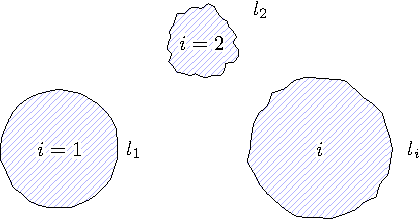
\includegraphics[scale=1.5]{img/lect4_ris1}
	\caption{Набор проводников в задаче}
	\label{fig:lect4:1}
\end{figure}

\subsubsection{Внутренняя задача}
\begin{figure}[H]
	\centering
	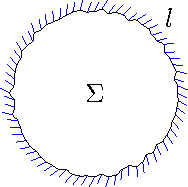
\includegraphics[scale=1.5]{img/lect4_ris2}
	\caption{Случай одного проводника}
	\label{fig:lect4:2}
\end{figure}
\subsubsection{Внешняя задача}
\begin{figure}[H]
	\centering
	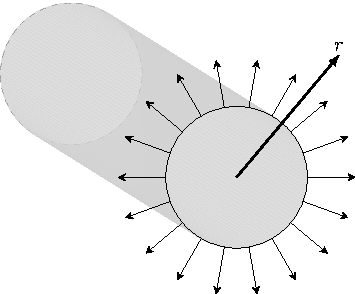
\includegraphics[scale=1.5]{img/lect4_ris3}
	\caption{Поле бесконечной проводящей нити}
	\label{fig:lect4:3}
\end{figure}

\begin{figure}[H]
	\centering
	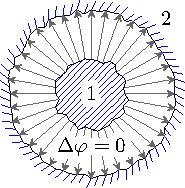
\includegraphics[scale=1.5]{img/lect4_ris4}
	\caption{Закрытая линия из двух проводников}
	\label{fig:lect4:4}
\end{figure}

\begin{figure}[H]
	\centering
	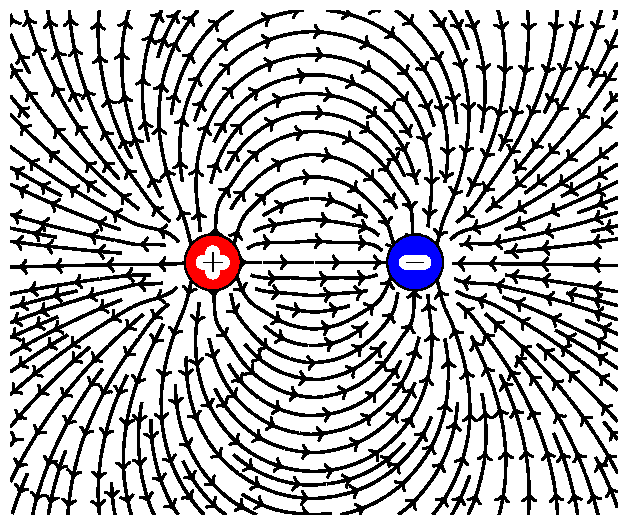
\includegraphics[scale=0.7]{img/lect4_ris5}
	\caption{Поле двухпроводной линии}
	\label{fig:lect4:5}
\end{figure}

\begin{figure}[H]
	\centering
	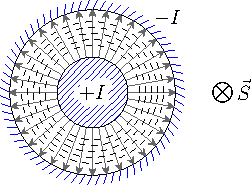
\includegraphics[scale=1.5]{img/lect4_ris6}
	\caption{Поле в коаксиальном кабеле}
	\label{fig:lect4:6}
\end{figure}
\subsection{TE и TM волны в идеальных линиях передачи закрытого типа}


\subsubsection{TE и TM волны в прямоугольном волноводе}

\begin{figure}[H]
	\centering
	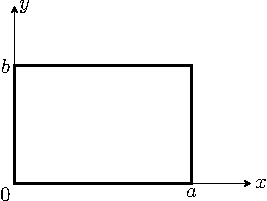
\includegraphics[scale=1.5]{img/lect4_ris7}
	\caption{Прямоугольный волновод}
	\label{fig:lect4:7}
\end{figure}

\begin{figure}[H]
	\centering
	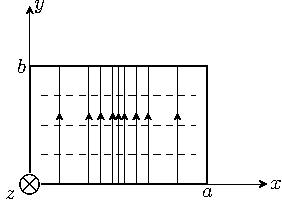
\includegraphics[scale=1.5]{img/lect4_ris8}
	\caption{Структура полей $\vec{E}$ и $\vec{H}$ ($\vec{H}$ изображено пунктиром)}
	\label{fig:lect4:8}
\end{figure}

\begin{figure}[H]
	\centering
	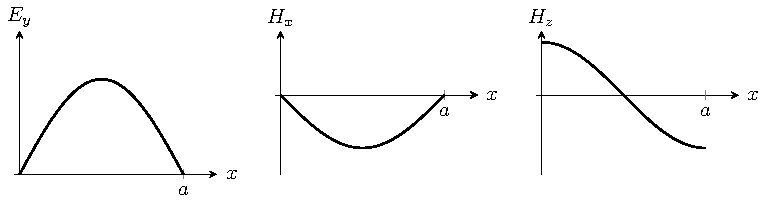
\includegraphics[width=\textwidth]{img/lect4_ris9}
	\caption{Поперечная структура полей $\vec{E}$ и $\vec{H}$ (мода TE$_{}$)}
	\label{fig:lect4:9}
\end{figure}

\begin{figure}[H]
	\centering
	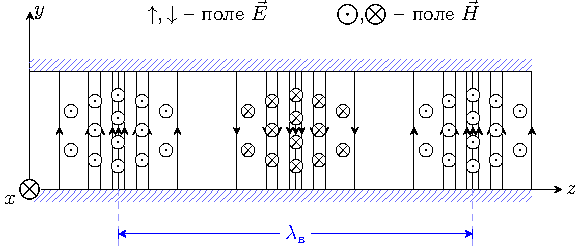
\includegraphics[width=\textwidth]{img/lect4_ris10}
	\caption{Продольная структура полей $\vec{E}$ и $\vec{H}$ (мода TE$_{}$)}
	\label{fig:lect4:10}
\end{figure}

\begin{figure}[H]
	\centering
	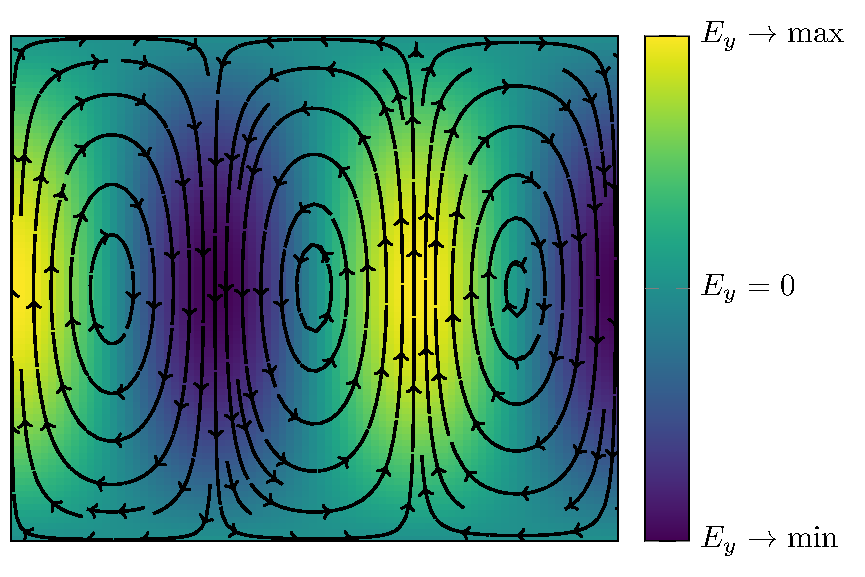
\includegraphics[scale=1]{img/lect4_ris11}
	\caption{Структура поля $\vec{H}$ (изображены силовые линии) и поля $\vec{E}$ (напряженность изображена цветом) волны TE$_{10}$ в прямоугольном волноводе}
	\label{fig:lect4:11}
\end{figure}